%%% VCU thesis/dissertation template file
\makeatletter
\let\my@xfloat\@xfloat
\makeatother

\documentclass[reqno]{vcuthesis}
\makeatletter
\def\@xfloat#1[#2]{
        \my@xfloat#1[#2]%
        \def\baselinestretch{1}%
        \@normalsize \normalsize
}
\makeatother
%%%%%%%%%%%%
% PACKAGES %
\usepackage{bm,amsmath,subfigure,graphicx,url,algorithm,algorithmicx,algpseudocode,booktabs}
\usepackage{tikz-cd,adjustbox,amsfonts,mathtools,tabularx,capt-of,longtable,comment,caption}
\usepackage[flushleft]{threeparttable}
\usepackage[top=1in,bottom=1in,right=1in,left=1in]{geometry}
\usepackage[backend=bibtex]{biblatex}
\usepackage[titletoc]{appendix}
\usepackage{pgfplots}
\pgfplotsset{compat=1.12}
\usepackage[linktocpage=true]{hyperref}
\usetikzlibrary{shapes.geometric,arrows,automata,positioning}
\usepackage{chngcntr}
\usepackage[final]{pdfpages}
\usepackage[explicit]{titlesec}

\newcommand{\iitem}{\item[-]}
\newcommand{\set}[1]{{\left\{#1\right\}}} 
\newcommand{\norm}[1]{{||#1||}} 
\newcommand{\st}{{\,|\,}} 
\newcommand{\reals}{{\mathbb{R}}}
\newcommand{\ints}{{\mathbb Z}}
\newcommand{\spa}[1]{\mathcal{#1}}
\newcommand\tab[1][1cm]{\hspace*{#1}}
\newcommand{\Rho}{\mathrm{P}}

%%%%%%%%%%%
\overfullrule=5pt
% BIBLIOGRAPHY %
\bibliography{references}
\renewcommand{\type}{Dissertation}
\renewcommand{\thetable}{\arabic{table}}
\newcommand{\comments}[1]{}
%%%%%%%%%%%

% EQUATIONS %
\numberwithin{equation}{chapter}
%%%%%%%%%%%

% DOCUMENT  %
\begin{document}
\counterwithin{figure}{chapter}
\counterwithin{algorithm}{chapter}
\counterwithin{table}{chapter}

\pagenumbering{roman}

\makeatletter
\newcommand\pagenumberingnoreset[1]{\gdef\thepage{\csname @#1\endcsname\c@page}}
\makeatother

\tikzstyle{decision} = [diamond, draw, text centered, inner sep=3pt]
\tikzstyle{block} = [rectangle, draw, fill=gray!20,text width=5em, text centered, rounded corners, minimum height=4em]
\tikzstyle{arrow} = [thick,->,>=stealth]

%%%%%%%%%%%
\newcommand{\thesisordissertation}{Dissertation}
\newcommand{\thesistitle}{\uppercase\expandafter{} Novel Support Vector Machines for Diverse Learning Paradigms}
\newcommand{\authorsname}{Gabriella Angela Melki}
\newcommand{\thesismonth}{September}
\newcommand{\graduatingyear}{2018}
\newcommand{\degree}{Doctor of Philosophy}
\newcommand{\pastdegreeone}{Ph.D. Candidate}
\newcommand{\pastdegreetwo}{MSc. Computer Science, Virginia Commonwealth University, 2016} % 897 in .cls
\newcommand{\committeechair}{Alberto Cano}
\newcommand{\committeechairtwo}{Sebastian Ventura}
\newcommand{\major}{Computer Science}
\newcommand{\school}{Virginia Commonwealth University}
\newcommand{\chairposition}{Assistant Professor}
\newcommand{\chairpositiontwo}{Professor}
\newcommand{\majortwo}{Computer Science \& Numerical Analysis}
\newcommand{\schooltwo}{University of C\'{o}rdoba}

\vspace*{10em}
\begin{center}
\thispagestyle{empty}
\copyright Gabriella Angela Melki, September {\graduatingyear}\\
All Rights Reserved.
\end{center}
\vspace*{\fill}
\maketitlepage

\setlength{\headheight}{12pt}
\pagenumberingnoreset{arabic}

\chapter{Novel OnLine SVM using Worst-Violators}
Due to the ever-growing nature of dataset sizes, the need for scalable and accurate machine learning algorithms has become evident. Stochastic gradient descent methods are popular tools used to optimize large-scale learning problems because of their generalization performance, simplicity, and scalability. This chapter proposes a novel stochastic, also known as online, learning algorithm for solving the L1 support vector machine (SVM) problem, named \textit{OnLine Learning Algorithm using Worst-Violators} (OLLAWV). Unlike other stochastic methods, OLLAWV eliminates the need for specifying the maximum number of iterations and the use of a regularization term. OLLAWV uses early stopping for controlling the size of the margin instead of the regularization term. The experimental study, performed under very strict nested cross-validation (a.k.a., double resampling), evaluates and compares the performance of this proposal with state-of-the-art SVM kernel methods that have been shown to outperform traditional and widely used approaches for solving L1-SVMs such as \textit{Sequential Minimal Optimization}. OLLAWV is also compared to $5$ other traditional non-SVM algorithms. The results over $23$ datasets show OLLAWV's superior performance in terms of accuracy, scalability, and model sparseness, making it suitable for large-scale learning.

\section{Online Learning Background}
This section defines the notation that will be used throughout the chapter, describes the support vector machine problem, and reviews related works on current popular solvers and online learning algorithms aimed at training support vector machines.

\begin{table}[t!]
\small \centering
\caption{Summary of notation used throughout the paper}\label{tab:ollawvNotation}
\begin{tabularx}{\textwidth}{l@{\extracolsep{\fill}}l}
\hline\noalign{\smallskip}
Definition & Notation\\ 
\noalign{\smallskip}\hline\noalign{\smallskip}
Number of Samples & $n$ \\
Number of Input Attributes & $d$ \\
Input Space & $\bm{X} \in \mathbb{R}^{n \times d}$ \\
Labels & $\bm{Y} \in \{-1,1\}^n$ \\
Sample $i$ & $\bm{x}_i = (x_{i1}, \ldots, x_{id}),\, \forall i \in \set{1,\ldots,n}$ \\
Sample Label $i$ & $y_i \in \set{-1,1},\, \forall i \in \set{1,\ldots,n}$ \\
\noalign{\smallskip}\hline\noalign{\smallskip}
Full Training Dataset & $\mathcal{D} = \{(\bm x_1,y_1), \ldots, \set{\bm x_i,y_i}, \ldots, (\bm x_n,y_n)\}$ \\
\noalign{\smallskip}\hline
\end{tabularx}
\end{table}

\subsection{Notation}\label{subsec:notation}
Let $\mathcal{D}$ be the full training dataset of $n$ $d$-dimensional samples. Let $\bm{Y} \in \mathcal{D}$ be a vector of $n$ labels corresponding to each sample, such that $\bm{Y} \in \set{-1,1}^n$. In the non-binary (more than two classes) classification cases, $\bm Y \in \ints^n$. Let $\bm{X} \in \mathcal{D}$ be a matrix consisting of $n$ samples that are $d$-dimensional, $\bm{X} \in \mathbb{R}^{n \times d}$. Table~\ref{tab:Notation} provides a summary of the notation used in this paper.

\subsection{Online Learning Methods}
\textbf{THIS MAYBE SHOULD GO IN THE SVM BACKGROUND}
\textbf{taken from Pegasos paper.}
Before indulging into the detailed description and analysis of Pegasos, we would like to draw connections to and put our work in context of some of the more recent work on SVM. For a more comprehensive and up-to-date overview of relevant work see the ref- erences in the papers cited below as well as the web site dedicated to kernel methods at http://www.kernel-machines.org . Due to the centrality of the SVM optimization problem, quite a few methods were devised and analyzed. The different approaches can be roughly divided into the following categories.
\textbf{taken from Pegasos paper.}

\begin{itemize}
\item \textbf{Interior Point (IP) methods:} IP methods (see for instance [7] and the references therein) cast the SVM learning task as a quadratic optimization problem subject to linear constraints. The constraints are replaced with a barrier function. The result is a sequence of uncon- strained problems which can be optimized very efficiently using Newton or Quasi-Newton methods. The advantage of IP methods is that the dependence on the accuracy ε is double logarithmic, namely, log(log(1/ε)). Alas, IP methods typically require run time which is cubic in the number of examples m. Moreover, the memory requirements of IP methods are O(m2) which renders a direct use of IP methods very difficult when the training set con- sists of many examples. It should be noted that there have been several attempts to reduce the complexity based on additional assumptions (see e.g. [15]). However, the dependence on m remains super linear. In addition, while the focus of the paper is the optimization problem cast by SVM, one needs to bear in mind that the optimization problem is a proxy method for obtaining good classification error on unseen examples. Achieving a very high accuracy in the optimization process is usually unnecessary and does not translate to a significant increase in the generalization accuracy. The time spent by IP methods for finding a sin- gle accurate solution may, for instance, be better utilized for trying different regularization values.

\item \textbf{Decomposition methods:} To overcome the quadratic memory requirement of IP methods, decomposition methods such as SMO [29] and SVM-Light [20] tackle the dual representa- tion of the SVM optimization problem, and employ an active set of constraints thus working on a subset of dual variables. In the extreme case, called row-action methods [8], the active set consists of a single constraint. While algorithms in this family are fairly simple to im- plement and entertain general asymptotic convergence properties [8], the time complexity of most of the algorithms in this family is typically super linear in the training set size m. Moreover, since decomposition methods find a feasible dual solution and their goal is to maximize the dual objective function, they often result in a rather slow convergence rate to the optimum of the primal objective function. (See also the discussion in [19].)

\item \textbf{Primal optimization: }Most existing approaches, including the methods discussed above, focus on the dual of Eq. (1), especially when used in conjunction with non-linear kernels. However, even when non-linear kernels are used, the Representer theorem [23] allows us to re-parametrize w as w = 􏱓αiyixi and cast the primal objective Eq. (1) as an un- constrained optimization problem with the variables α1 , . . . , αm (see Sec. 4). Tackling the primal objective directly was studied, for example, by Chapelle [10], who considered us- ing smooth loss functions instead of the hinge loss, in which case the optimization problem becomes a smooth unconstrained optimization problem. Chapelle then suggested using var- ious optimization approaches such as conjugate gradient descent and Newton’s method. We take a similar approach here, however we cope with the non-differentiability of the hinge- loss directly by using sub-gradients instead of gradients. Another important distinction is that Chapelle views the optimization problem as a function of the variables αi. In contrast, though Pegasos maintains the same set of variables, the optimization process is performed with respect to w, see Sec. 4 for details.

\item \textbf{Stochastic gradient descent:} The Pegasos algorithm is an application of a stochastic sub- gradient method (see for example [25,34]). In the context of machine learning problems, the efficiency of the stochastic gradient approach has been studied in [26,1,3,27,6,5]. In particular, it has been claimed and experimentally observed that, “Stochastic algorithms yield the best generalization performance despite being the worst optimization algorithms”. This claim has recently received formal treatment in [4,32].
Two concrete algorithms that are closely related to the Pegasos algorithm and are also variants of stochastic sub-gradient methods are the NORMA algorithm [24] and a stochas- tic gradient algorithm due to Zhang [37]. The main difference between Pegasos and these variants is in the procedure for setting the step size. We elaborate on this issue in Sec. 7. The convergence rate given in [24] implies that the number of iterations required to achieve ε-accurate solution is O(1/(λ ε)2). This bound is inferior to the corresponding bound of Pe- gasos. The analysis in [37] for the case of regularized loss shows that the squared Euclidean distance to the optimal solution converges to zero but the rate of convergence depends on the step size parameter. As we show in Sec. 7, tuning this parameter is crucial to the success of the method. In contrast, Pegasos is virtually parameter free. Another related recent work is Nesterov’s general primal-dual subgradient method for the minimization of non-smooth functions [28]. Intuitively, the ideas presented in [28] can be combined with the stochastic regime of Pegasos. We leave this direction and other potential extensions of Pegasos for future research.

\item \textbf{Cutting Planes Approach:} Recently, Joachims [21] proposed SVM-Perf, which uses a cut- ting planes method to find a solution with accuracy ε in time O(md/(λε2)). This bound was later improved by Smola et al [33] to O(md/(λε)). The complexity guarantee for Pe- gasos avoids the dependence on the data set size m. In addition, while SVM-Perf yields very significant improvements over decomposition methods for large data sets, our experiments (see Sec. 7) indicate that Pegasos is substantially faster than SVM-Perf.
\end{itemize}

\section{OnLine Learning Algorithm using Worst-Violator}\label{sec:contribution}
OLLAWV is an iterative, online learning algorithm for solving the L1-SVM problem using a novel model update procedure while implementing a self-stopping condition. The inspiration behind OLLAWV came from~\cite{kecman2016fast} which presented a generic online learning algorithm tailored not only for SVMs, but also for various other popular classifiers that use different risk functions, with or without a regularization term. The difference, novelty, and advantage of OLLAWV resides in its iterative method, where the weight $\alpha_i$ of the most violating sample i.e., of the \textit{worst-violator}, is only updated in each iteration. A worst violating sample is defined as the sample that has the largest error with respect to the current decision function. Rather than randomly selecting samples to update per iteration, OLLAWV selects (without replacement) the most incorrectly classified sample and updates the model accordingly. By iteratively updating the model using only the worst-violator, the model is essentially finding its support vectors, as well as implicitly defining a stopping criterion. If there are no more violating samples, the algorithm terminates, eliminating the need to define the number of iterations for an algorithm to perform before returning the model, as is the case with most state-of-the-art online algorithms. 

At every iteration, the algorithm selects a worst violating sample that has not been previously chosen, stores its index in vector $\bm S$, and then updates the model. Equation~\ref{eq:wv} shows the method for selecting the worst-violator, where $yo \in \reals$ is the error value, $wv \in \set{1, \ldots, n}$ is the error value's index, $\bm o \in \reals^n$ is the decision function output, and $\neg$ is the `not' symbol. For the L1-SVM, an error value will always be negative which is why the minimum function is used (i.e. the most negative output value or incorrectly classified sample). The worst violating sample becomes the model's support vector because its weight is updated and non-zero. Therefore, the number of iterations of OLLAWV is equal to the number of support vectors that the resulting model has. This is an interesting property of OLLAWV; if the number of iterations is set beforehand, one is implicitly setting a bound on the number of support vectors. 
\begin{equation}
[yo, wv] = \min \set{y_{wv} \cdot o_{wv}},\, \forall wv \in \set{\neg \bm S}
\label{eq:wv}
\end{equation}

Algorithm~\ref{alg:ollawv} lists OLLAWV's pseudocode and Figure~\ref{fig:ollawv} illustrates the steps taken by OLLAWV. First, the model parameters ($\bm \alpha$, $b$, $\bm S$) and the algorithm variables ($\bm o$, iteration counter ($t$), initial worst-violator index $wv$ and it's error $yo$) are first initialized. The worst-violator with respect to the current hyperplane is then found and the model parameters are updated. Once no more violating samples are found or the maximum number of iterations is reached, the model is returned.

OLLAWV performs stochastic gradient descent on the primal L1-SVM objective function given below:
\begin{equation}
\label{eq:l1svm}
\min\limits_{\bm{w} \in \mathcal{H}_o \times \reals} R {\,\,} = {\,\,} \frac{1}{2}||\bm{w}||^2 + C\sum_{i=1}^n \max \set{0, 1 - y_i o_{(w)}(\bm{x}_i)},
\end{equation}
where $o_{(w)}(\bm{x}_i) = \langle\bm w, \bm x_i\rangle$ is a linear predictor, with the bias term excluded for simplicity. Note that the loss function used in Equation~\ref{eq:l1svm} is non-differentiable, but it has a subgradient due to a knick-point at $yo = 1$. The loss function's gradient after the knick-point equals zero, which leads to a sparse model. Hence, when the value of $yo \geq 1$ the loss is zero, and for $yo < 1$ the loss increases linearly. The subgradient of the above cost function is given by:
\begin{equation}
\label{eq:subgrful}
\frac{\partial R}{\partial \bm w} = \begin{cases} 
						\bm w - C \sum_{i=1}^n y_i \bm{x_i} & y_i o_i < 1 \\
						\bm w & \text{otherwise.}
						\end{cases}
\end{equation}
In the stochastic case, the calculation of the gradient needed for the weight update, is \textit{pattern based}, not \textit{epoch based} as in batch gradient descent. It has been shown~\cite{Kecman2001} that the ideal gradient is equal to the sum of the gradients calculated after each sample is presented for fixed weights during the whole epoch. Thus, the stochastic update of $\bm w$ from the subgradient shown in Equation~\ref{eq:subgrful} becomes:
\begin{align*}
\bm w &\leftarrow \bm w - \eta \frac{\partial R}{\partial \bm w} \\
\bm w &\leftarrow \bm w + \eta \begin{cases} 
															C y_i \bm{x_i} - \bm w & y_i o_i < 1 \\
															-\bm w & \text{otherwise},
													 \end{cases}
\end{align*}
where $\eta > 0 \in \reals $ is the learning rate. According to the Representer Theorem, a vector $\bm \alpha \in \reals^n$ exists such that $\bm w = \sum_{i=1}^n \alpha_i \phi(\bm x_i)$ is an optimal solution to Equation~\ref{eq:l1svm}, where $\phi(\cdot)$ is a mapping from feature space to Hilbert space~\cite{Shalev2014}. On the basis of the Representer Theorem, Equation~\ref{eq:l1svm} can be optimized with respect to $\bm \alpha$ instead of $\bm w$. By expressing $\bm w$ this way and mapping input sample $\bm{x_i}$ to $\phi(\bm{x_i})$, the kernelized SGD update becomes:
\begin{equation*}
\centering
\sum_{i=1}^n \alpha_i \phi(\bm x_i) \leftarrow \sum_{i=1}^n \alpha_i \phi(\bm x_i) + \eta \begin{cases} 
															C y_i \phi(\bm{x_i}) - \sum_{i=1}^n \alpha_i \phi(\bm x_i) & y_i o_i < 1 \\[5pt]
															-\sum_{i=1}^n \alpha_i \phi(\bm x_i) & \text{otherwise}.
													 \end{cases}
\end{equation*}
However, OLLAWV optimizes in a stochastic manner, resulting in the following update:
\begin{align*}
&\forall i: \alpha_i \phi(\bm x_i) \leftarrow \alpha_i \phi(\bm x_i) + \eta \begin{cases} 
																													(Cy_i\phi(\bm{x_i}) - \alpha_i \phi(\bm x_i)) & y_i o_i < 1 \\
																													(- \alpha_i \phi(\bm x_i)) & \text{otherwise}
																													 \end{cases} \\							
&\forall i: \alpha_i \leftarrow \alpha_i + \eta \begin{cases} 
																(Cy_i - \alpha_i) & y_i o_i < 1 \\
																(- \alpha_i) & \text{otherwise}.
															\end{cases} 
\end{align*}
The case when the worst violating sample is correctly classified $yo \geq 1$ is OLLAWV's termination condition, i.e. is used as the stopping criterion in the algorithm. Hence the update for $\bm \alpha$ is reduced to the following:
\begin{equation}
\label{eq:alphaupdate}
\forall i: \alpha_i \leftarrow \alpha_i + \eta(Cy_i - \alpha_i)
\end{equation}
If the bias term $b$ is included in Equation~\ref{eq:l1svm}, it's stochastic update is as follows:
\begin{equation}
\label{eq:upbias}
\forall i: b \leftarrow b + \eta \frac{C y_i}{n}
\end{equation}

\begin{figure}[t!]
\centering
\begin{minipage}{0.49\textwidth}
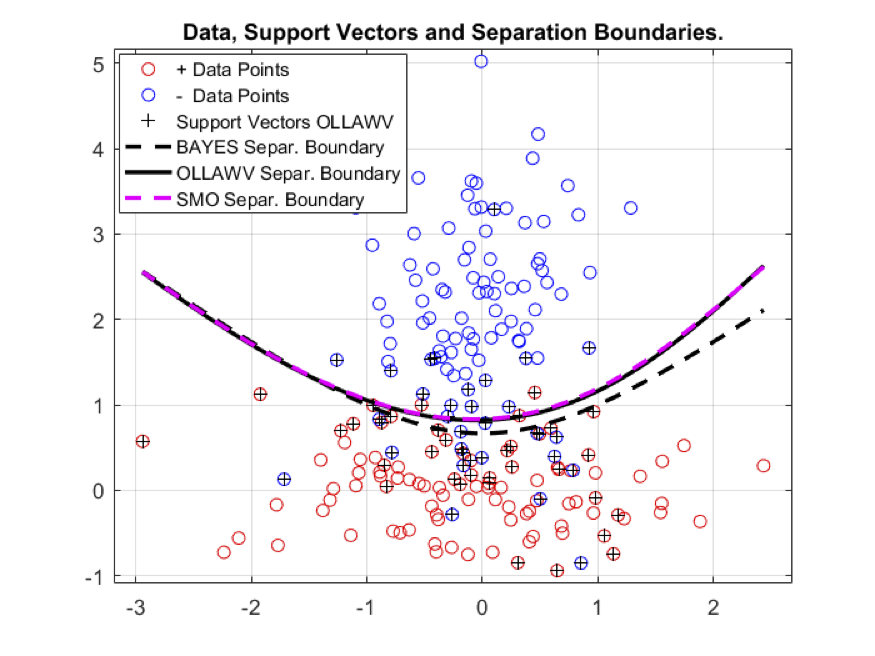
\includegraphics[width=\textwidth]{../figures/OLLAWVSeparation.png}
\end{minipage}
\begin{minipage}{0.49\textwidth}
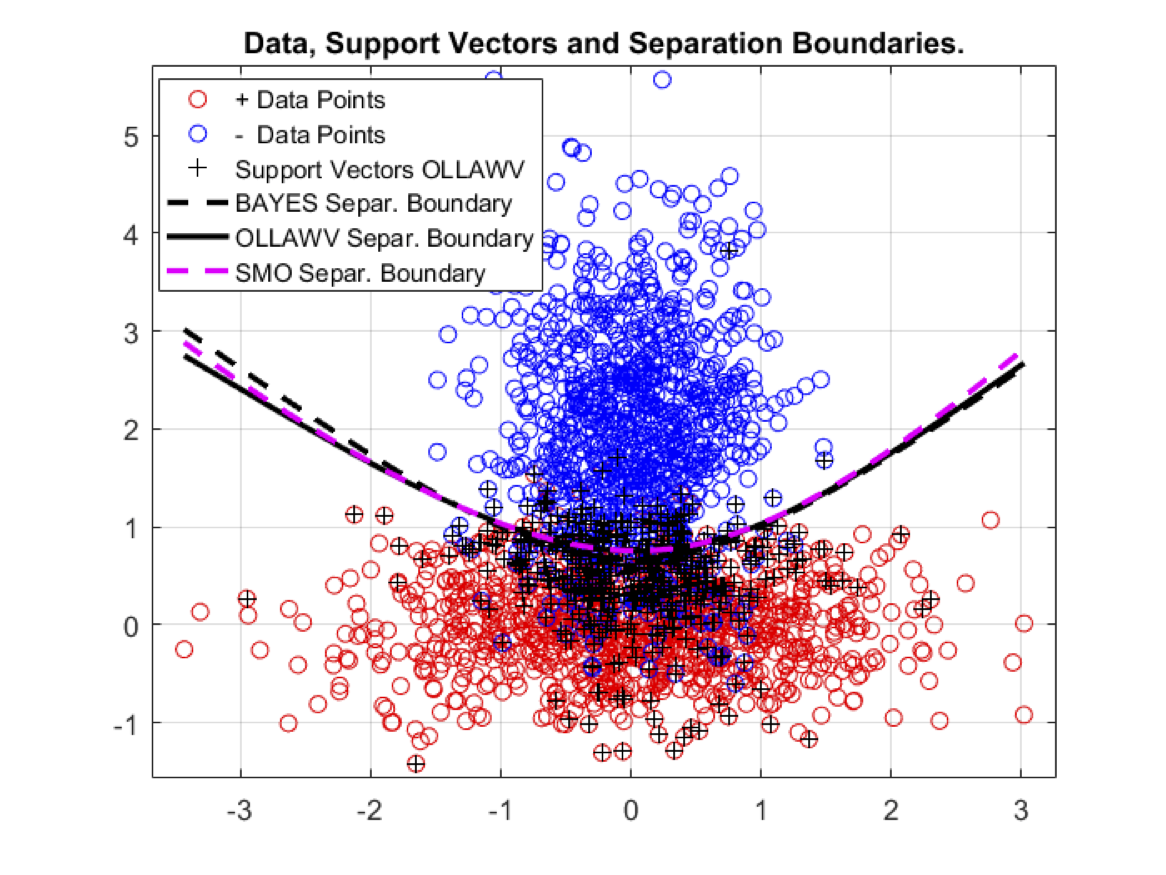
\includegraphics[width=\textwidth]{../figures/SeparationOLLAWV2000.png}
\end{minipage}
\caption{A case of classifying 2-dimensional normally distributed data with different covariance matrices, (left) for 200 and (right) 2000 data points. The theoretical separation boundary (denoted as the Bayes Separation Boundary) is quadratic and is shown as the dashed black curve. The other two separation boundaries shown are the ones obtained by OLLAWV and SMO (implemented within LIBSVM), respectively. In this particular case (left), the difference between the OLLAWV boundary and the SMO boundary is hardly visible. The case presented on the right shows that, with an increase of training samples, the OLLAWV and SMO boundaries converge to the theoretical Bayesian solution.}
\label{fig:ollawvseparation}
\end{figure}

In this experimental study, $\eta = 2/\sqrt{t}$ is used, where $t$ is the current iteration; however, other learning rates such as $\eta = 1/t$ can also be used. Let $\Lambda = \eta Cy_i$ and $\Rho = \eta \alpha_i$ be the update parameters for OLLAWV, and the $\bm \alpha$ update can be expressed as: $\alpha_i \leftarrow \alpha_i + (\Lambda - \Rho)$. Note that $\Lambda$ is the update resulting from the loss function and $\Rho$ is derived from the regularizer term in Equation~\ref{eq:l1svm}. In the case of OLLAWV, $\Rho = 0$ because samples are never updated more than once and their initial $\alpha$ value is always $0$. It is important to note that in OLLAWV's case, $\Lambda$ never equals $0$ because the samples being updated are worst-violators, meaning they are misclassified or incur some loss. The values of the decision function (output vector $\bm o \in \reals^n$ in Algorithm~\ref{alg:ollawv}), from which a worst-violator is found, changes per iteration based on the influence of the support-vectors that have been previously updated. From Equation~\ref{eq:output}, the output vector update becomes the following: 
\begin{equation}
\label{eq:upoutput}
\bm o \leftarrow \bm o + \Lambda*\mathcal{K}\left(\bm{x}_{\neg \bm S},\, \bm{x}_{wv}, \gamma \right) + B
\end{equation}
where $\mathcal{K}(\cdot)$ is the Gaussian radial basis function (RBF) kernel, $\gamma \in \reals$ is it's parameter, and $B = (\Lambda * \beta)/n$ denotes the bias update. Only non-support vector output values are calculated per iteration, as denoted by $\bm x_{\neg \bm S}$ in the kernel function, because samples are never selected to be updated more than once. Because the output values scale with the $C$ value, the stopping criteria for OLLAWV is also set to scale with $C$, rather than the classic formulation $y_i o_i \geq 1$. If the value of $C$ is very large, $y_i o_i$ will never be greater than 1 and the algorithm will never terminate. Therefore, the stopping criteria is set to be $y_i o_i \geq M$, where $M \in \reals$ is a scaled value of $C$. For the $B$ calculation in Equation~\ref{eq:upoutput}, $\beta \in \set{0,1}$ indicates whether the bias term is to be used. If $b$ is not a part of the model, it should be omitted from Equations~\ref{eq:output} and~\ref{eq:upoutput} by setting $\beta = 0$, otherwise $\beta = 1$. 

OLLAWV is a stochastic gradient method (SGM) that has a convex cost function. Its learning rate coefficient can decrease linearly or semi-linearly during the learning stage. Hence, OLLAWV shares the complexity characteristics of SGM methods. Primarily, it can achieve linear convergence, making it a particularly convenient and practical method for solving very large machine learning problems. OLLAWV also works over a cost function without local minima, always leading towards the global minimum, even though it stops the learning process as soon as all samples are outside the prescribed margin. Figure~\ref{fig:ollawvseparation} shows the decision boundaries achieved by OLLAWV versus SMO (implemented within LIBSVM) and Bayes for toy datasets. 
\begin{figure}
\centering
\small
\begin{algorithm}[H]
\small
\caption{OnLine Learning Algorithm using Worst-Violators (OLLAWV)}
\label{alg:ollawv}
\begin{algorithmic}[1]
\renewcommand{\algorithmicrequire}{\textbf{Input:}}
\renewcommand{\algorithmicensure}{\textbf{Output:}}
\Require $\mathcal{D}$, $C$, $\gamma$, $\beta$, $M$
\Ensure  $\bm \alpha$, $b$, $\bm S$
\State $\bm \alpha \leftarrow \bm 0,\, b \leftarrow 0, \bm S \leftarrow \bm 0$ \Comment{Initialize OLLAWV model parameters}
\State $\bm o \leftarrow \bm 0,\, t \leftarrow 0$ \Comment{Initialize the output vector and iteration counter}
\State $wv \leftarrow 0,\, yo \leftarrow y_{wv}*\bm{o}_{wv}$ \Comment{Initialize hinge loss error and worst-violator index}
\While {$yo < M$}
\State $t \leftarrow t + 1$
\State $\eta \leftarrow 2/\sqrt{t}$ \Comment{Learning rate}
\State 
\State $\Lambda \leftarrow \eta*C*y_{wv}$ \Comment{Calculate hinge loss update}
\State $B \leftarrow \left(\Lambda*\beta\right)/n$ \Comment{Calculate bias update}
\State $\bm o \leftarrow \bm o + \Lambda*\mathcal{K}\left(\bm{x}_{\neg \bm S},\, \bm{x}_{wv}, \gamma \right) + B$ \Comment{Update output vector}
\State $\bm \alpha_{wv} \leftarrow \bm \alpha_{wv} + \Lambda$ \Comment{Update worst-violator's alpha value}
\State $b \leftarrow b + B$ \Comment{Update bias term}
\State
\State $\bm S_t \leftarrow wv$ \Comment{Save index of worst-violator}
\State $\left[yo,\, wv\right] \leftarrow \min\limits_{wv \in \set{\neg \bm S}}\set{y_{wv} \cdot o_{wv}}$ \Comment{Find the worst-violator}
\EndWhile 
\end{algorithmic} 
\end{algorithm}
\begin{minipage}{\textwidth}
\small
\adjustbox{scale=0.9}{
\begin{tikzpicture}[%
    node distance=4cm,
    on grid,
    auto
]
\node[block](A) {Initialize training variables};
\node(B)[block, right of=A, text width=6em] {Calculate updates based on worst-violator and current decision boundary};
\draw[arrow] (A) -- (B);
\node(C)[block, right of=B,text width=6.3em] {Update output vector, worst-violator's alpha, \& bias term};
\draw[arrow] (B) -- (C);
\node(D) [decision,right of=C,fill=gray!55,text width=2cm]{while errors exist};
\draw[arrow] (C) -- (D);
\node(E) [block,right of=D]{return $\bm \alpha,\, b, \bm S$};
\draw[arrow] (D) -- node {no} (E);
\draw[arrow] (D.south) --+(0,-0.35cm) -| (B.south) node[below,pos=0.25] {yes} ;
\end{tikzpicture}}
\caption{A summary of the steps performed by OLLAWV. The model parameters ($\bm \alpha$, $b$, $\bm S$) and the algorithm variables ($\bm o$, $t$, $wv$, and $yo$) are first initialized. The worst-violator with respect to the current hyperplane is then found and the model parameters are then updated. Once no more violating samples are found, the model is returned.}
\label{fig:ollawv}
\end{minipage}
\end{figure}

\section{Experimental Environment, Results, and Analysis}\label{sec:exp}
This section presents two experimental setups of our contribution against other state-of-the-art algorithms on $23$ different benchmark datasets. The first study, presented in Section~\ref{subsec:expsvm}, compares OLLAWV to two other SVM kernel methods, and the second compares OLLAWV to $5$ non-SVM methods, shown in Section~\ref{subsec:nonsvmexp}. In each section, the experimental setups are first described and the state-of-the-art methods are listed. The results and statistical analysis~\cite{Derrac2011} are then presented and analyzed. The main aim of the experiments is to compare our contribution to other support vector machine solvers that have been shown to surpass popular and widely used SVM kernel methods in terms of memory consumption, runtime, and accuracy. The supplemental experimental study in~\ref{subsec:nonsvmexp} was conducted to emphasizes the better performance of OLLAWV against non-SVM algorithms.
\begin{table}[t!]
\caption{Datasets}
\footnotesize
\centering
\label{tab:Dataset}
\begin{tabularx}{0.7\textwidth}{l@{\extracolsep{\fill}}rrr}
\hline\noalign{\smallskip}
Dataset & \# Samples & \# Attributes & \# Classes \\
\noalign{\smallskip}\hline\noalign{\smallskip}
\textbf{\textit{small datasets}} & \\
iris & 150 & 4 &  3  \\ 
teach & 151 & 5 &  3  \\ 
wine & 178 & 13 &  3  \\ 
cancer & 198 & 32 &  2  \\ 
sonar & 208 & 60 &  2  \\ 
glass & 214 & 9 &  6  \\ 
vote & 232 & 16 &  2  \\ 
heart & 270 & 13 &  2  \\ 
dermatology & 366 & 33 &  6  \\ 
prokaryotic & 997 & 20 &  3  \\ 
eukaryotic & 2,427 & 20 &  2  \\ 
\textbf{\textit{medium datasets}} & \\
optdigits & 5,620 & 64 &  10  \\ 
satimage & 6,435 & 36 &  6  \\ 
usps & 9,298 & 256 &  10  \\ 
pendigits & 10,992 & 16 &  10  \\ 
reuters & 11,069 & 8,315 &  2  \\ 
letter & 20,000 & 16 &  26  \\ 
\textbf{\textit{large datasets}} & \\
adult & 48,842 & 123 &  2  \\ 
w3a & 49,749 & 300 &  2  \\ 
shuttle & 58,000 & 7 &  7  \\ 
web (w8a) & 64,700 & 300 &  2  \\ 
ijcnn1 & 141,691 & 22 &  2  \\ 
intrusion & 5,209,460 & 127 &  2  \\  
\noalign{\smallskip}\hline
\end{tabularx}
\end{table}

Table~\ref{tab:Dataset} presents a summary of the $23$ datasets used throughout the experiments, where the number of attributes (dimensionality), classes, and samples are shown. The datasets used and the results obtained are divided into three groups: \textit{small}, \textit{medium} and \textit{large}. The datasets were obtained from the UCI Machine Learning repository\footnote{http://archive.ics.uci.edu/ml/index.php}~\cite{Lichman:2013}, and the LibCVM\footnote{http://c2inet.sce.ntu.edu.sg/ivor/cvm.html}~\cite{tsang2005core} and LIBSVM\footnote{https://www.csie.ntu.edu.tw/~cjlin/libsvmtools/datasets/}~\cite{CC01a} sites. 

\subsection{SVM Experimental Setup}\label{subsec:expsvm}
The experimental setup was designed to evaluate differences in performance of the proposed OLLAWV method against the state-of-the-art algorithms: \textit{Minimal Norm SVM} (MNSVM) \cite{strack2013geometric} and \textit{Non-Negative Iterative Single Data Algorithm} (NNISDA)~\cite{zigic2016}. These algorithms were chosen because they have shown considerable performance in runtime, memory consumption, and accuracy against the popular and widely used LIBSVM and LibCVM pagackes. In~\cite{strack2013geometric}, it was shown that MNSVM outperforms both the L1 and L2 implementations of LIBSVM, and BVM embedded in LibCVM. NNISDA was then compared to MNSVM in~\cite{zigic2016}, and showed an added improvement in runtime performance. MNSVM was implemented in an open source C++ framework called ``GSVM – Command Line Tool for Geometric SVM Training\footnote{Strack-Kecman, https://github.com/strackr/gsvm}''. Both, NNISDA and OLLAWV were implemented as additional modules within Strack-Kecman's code, keeping the experimental environment controlled for all three algorithms. The experiments for all methods were run on the same computer containing two Intel Xeon X5680 CPUs (6-core, 3.33 GHz) and 96 GB of RAM.

Experiments were performed using double, or nested, $5$-fold cross-validation in order to objectively evaluate the models' performances and tune hyper-parameters~\cite{varma2006bias,wu2017two}. In the outer loop, the data are separated into $5$ equally sized folds and each part is held out in turn as the test set, and the remaining four parts are used as the training set. In the inner loop, $5$-fold cross-validation is also used over the training set assigned by the outer loop, where the best hyper-parameters are chosen. The best model obtained by the inner loop is then applied on the outer loop's test set. This procedure ensures the model's performance is not optimistically biased as when using a single loop of $k$-fold cross-validation. It ensures the class labels of the test data will not be seen when tuning the hyper-parameters, which is consistent with real-world applications. Obviously, such a rigorous procedure is computationally expensive, but the goal is to fairly compare different classification models on the same data sets, with the same cross-validation procedure, and hyper-parameters. First, the datasets were normalized by linear transformation of the feature values to the range $[0,1]$. Then, the training process, also involving model selection using pattern search, was performed. The best hyper-parameters were chosen from the following $8 \times 8$ possible combinations, shown in Equations~\eqref{eq:paramC} and~\eqref{eq:paramG}, and were also used for the competing SVM methods.
\begin{subequations}
\label{eq:hyperparam}
\begin{align}
C \in \set{4^n}, & \,\,\,\,\,n = \set{-2, \ldots, 5} \label{eq:paramC}\\
\gamma \in \set{4^n},  & \,\,\,\,\,n = \set{-5, \ldots, 2} \label{eq:paramG}
\end{align}
\end{subequations}
The $\gamma$ parameter refers to that of the Gaussian RBF kernel, given by:
\begin{equation}
\label{eq:rbf}
\mathcal{K}(\bm{x_i},\bm{x_j}) = e^{-\gamma\norm{\bm{x_i} - \bm{x_j}}^2}.
\end{equation}

To deal with multi-class classification problems, the one-vs-one, or pairwise, approach was used. The pairwise training procedure trains $c(c - 1)/2$ binary classifiers, a classifier for each possible pair of classes, where $c$ is the number of classes. During the prediction phase, a voting scheme is used where all $c(c - 1)/2$ models predict an unseen data sample and the class that received the highest number of votes is considered to be the sample’s true class.

\begin{table}[t!]
\centering
\caption{Comparison of OLLAWV vs. NNISDA and MNSVM}
\scriptsize
\label{tab:results}
\resizebox{\textwidth}{!}{\begin{tabularx}{\textwidth}{l@{\extracolsep{\fill}}cccrrrccc}
\noalign{\smallskip}\hline\noalign{\smallskip}
\multicolumn{1}{l}{Dataset} & \multicolumn{3}{c}{Accuracy (\%)} & \multicolumn{3}{c}{Runtime (s)} & \multicolumn{3}{c}{Support Vectors (\%)} \\
\cmidrule(lr){2-4}
\cmidrule(lr){5-7}
\cmidrule(lr){8-10} 
 & OLLAWV & NNISDA & MNSVM & OLLAWV & NNISDA & MNSVM & OLLAWV & NNISDA & MNSVM \\
\noalign{\smallskip}\hline\noalign{\smallskip}
\textbf{\textit{small datasets}} & & & & & & & & & \\
iris & \textbf{97.33} & 94.00 & 96.67 & \textbf{0.05} & 0.27 & 3.57 & \textbf{13.50} & 40.20 & 29.80 \\
teach & 52.32 & 52.31 & \textbf{52.95} & \textbf{0.12} & 0.44 & 8.85 & \textbf{69.19} & 99.80 & 87.40 \\
wine & \textbf{98.87} & 96.60 & 96.60 & \textbf{0.28} & 0.43 & 4.84 & \textbf{15.02} & 44.40 & 48.60 \\
cancer & 80.36 & \textbf{81.86} & 81.38 & \textbf{0.49} & 0.85 & 4.46 & \textbf{42.79} & 83.80 & 89.60 \\
sonar & \textbf{92.32} & 89.48 & 87.57 & \textbf{0.59} & 0.98 & 3.03 & \textbf{31.26} & 73.00 & 66.00 \\
glass & \textbf{72.41} & 67.81 & 69.30 & \textbf{0.46} & 1.01 & 11.94 & \textbf{62.84} & 90.80 & 87.60 \\
vote & \textbf{96.54} & 96.11 & 93.99 & \textbf{0.26} & 0.46 & 1.49 & \textbf{13.36} & 33.20 & 34.00 \\
heart & 82.22 & \textbf{83.33} & \textbf{83.33} & \textbf{0.50} & 0.91 & 6.45 & \textbf{37.69} & 73.00 & 82.00 \\
dermatology & 97.82 & \textbf{98.36} & \textbf{98.36} & \textbf{1.62} & 2.47 & 11.68 & \textbf{36.94} & 59.00 & 59.80 \\
prokaryotic & 88.96 & 88.86 & \textbf{88.97} & \textbf{6.09} & 10.64 & 50.86 & \textbf{29.01} & 51.20 & 49.00 \\
eukaryotic & 77.38 & 79.56 & \textbf{81.21} & 61.95 & \textbf{49.16} & 342.76 & \textbf{54.11} & 76.40 & 72.60 \\
\textbf{\textit{medium datasets}} & & & & & & & & & \\
optdigits & 99.11 & 99.29 & \textbf{99.31} & \textbf{411} & 528 & 787 & \textbf{28.64} & 31.60 & 30.60 \\
satimage & 91.66 & \textbf{92.39} & 92.35 & 1,334 & \textbf{687} & 1,094 & \textbf{20.72} & 45.00 & 44.80 \\
usps & 97.49 & 98.05 & \textbf{98.24} & 10,214 & \textbf{5,245} & 7,777 & \textbf{11.22} & 29.40 & 28.00 \\
pendigits & 99.56 & \textbf{99.62} & 99.61 & \textbf{723} & 909 & 1,500 & \textbf{10.27} & 17.60 & 16.60 \\
reuters & 98.03 & \textbf{98.08} & 97.99 & \textbf{954} & 1,368 & 1,657 & \textbf{8.770} & 18.20 & 18.60 \\
letter & 96.99 & 99.11 & \textbf{99.13} & \textbf{5,259} & 12,009 & 26,551 & \textbf{43.56} & 57.60 & 56.60 \\
\textbf{\textit{large datasets}} & & & & & & & & & \\
adult & 84.75 & 85.07 & \textbf{85.13} & \textbf{21,025} & 72,552 & 123,067 & \textbf{34.66} & 56.00 & 56.60 \\
w3a & \textbf{98.86} & 98.82 & 98.82 & \textbf{6,532} & 15,951 & 24,562 & \textbf{3.270} & 14.60 & 12.40 \\
shuttle & 99.77 & 99.83 & \textbf{99.87} & \textbf{2,833} & 7,420 & 45,062 & \textbf{2.010} & 6.00 & 16.40 \\
web & 98.94 & \textbf{99.00} & 99.00 & \textbf{12,067} & 30,583 & 38,040 & \textbf{4.320} & 13.20 & 10.80 \\
ijcnn1 & 98.31 & 99.34 & \textbf{99.41} & \textbf{162,587} & 296,917 & 370,144 & 16.36 & 11.00 & \textbf{7.600} \\
intrusion & \textbf{99.77} & 99.67 & 99.66 & \textbf{2,402,804} & 4,646,810 & 3,772,113 & \textbf{0.780} & 2.000 & 1.700 \\
\noalign{\smallskip}\hline\noalign{\smallskip}
Average & \textbf{91.29} & 91.15 & 91.25 & \textbf{114,209} & 221,350 & 191,861 & \textbf{25.66} & 44.65 & 43.79 \\
Ranks & \textbf{1.739} & 2.022 & 2.239 & \textbf{1.217} & 1.913 & 2.869 & \textbf{1.087} & 2.609 & 2.304 \\
\noalign{\smallskip}\hline\noalign{\smallskip}
\end{tabularx}}
\\ \vspace{2em}
\begin{minipage}{0.3\textwidth}
\centering
\resizebox{0.9\textwidth}{!}{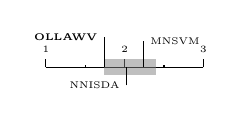
\begin{tikzpicture}
\draw (1,0) -- (3,0);
\foreach \x in {1,2,3} {
\draw (\x, 0) -- ++(0,.1) node [above,scale=0.7] {\tiny \x};
\ifthenelse{\x < 3}{\draw (\x+.5, 0) -- ++(0,.03);}{}
}

\coordinate (c0) at (1.7391,0);
\coordinate (c1) at (2.0217,0);
\coordinate (c2) at (2.2391,0);

\node (l0) at (c0) [above left=.25cm and 0cm, align=right,scale=0.7] {\tiny \textbf{OLLAWV}};
\node (l1) at (c1) [below left=.1cm and 0cm, align=right,scale=0.7] {\tiny NNISDA};
\node (l2) at (c2) [above right=.2cm and 0cm, align=right,scale=0.7] {\tiny MNSVM};

\fill[fill=gray,fill opacity=0.5] (1.7391,-0.1) rectangle (2.3991,0.1);

\foreach \x in {0,1,2} {
\draw (l\x) -| (c\x);
};
\end{tikzpicture}}
\captionsetup{width=0.8\linewidth}
\captionof{figure}{Bonferroni-Dunn test for Accuracy}\label{fig:BonfDunnacc}
\end{minipage}
\hspace{0.5em}
\begin{minipage}{0.3\textwidth}
\centering
\resizebox{0.9\textwidth}{!}{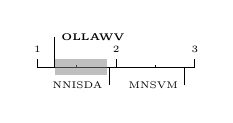
\begin{tikzpicture}
\draw (1,0) -- (3,0);
\foreach \x in {1,2,3}{
\draw (\x, 0) -- ++(0,.1) node [above,scale=0.7] {\tiny \x};
\ifthenelse{\x < 3}{\draw (\x+.5, 0) -- ++(0,.03);}{}
}

\coordinate (c0) at (1.2174,0);
\coordinate (c1) at (1.913,0);
\coordinate (c2) at (2.8696,0);

\node (l0) at (c0) [above right=.25cm and 0cm, align=right,scale=0.7] {\tiny \textbf{OLLAWV}};
\node (l1) at (c1) [below left=.1cm and 0cm, align=right,scale=0.7] {\tiny NNISDA};
\node (l2) at (c2) [below left=.1cm and 0cm, align=right,scale=0.7] {\tiny MNSVM};

\fill[fill=gray,fill opacity=0.5] (1.2174,-0.1) rectangle (1.8774,0.1);

\foreach \x in {0,1,2} {
\draw (l\x) -| (c\x);
};
\end{tikzpicture}}
\captionsetup{width=0.8\linewidth}
\captionof{figure}{Bonferroni-Dunn test for Runtime}\label{fig:BonfDunncpu}
\end{minipage}
\hspace{0.5em}
\begin{minipage}{0.3\textwidth}
\centering
\resizebox{0.9\textwidth}{!}{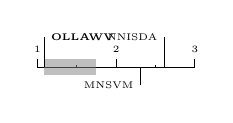
\begin{tikzpicture}
\draw (1,0) -- (3,0);
\foreach \x in {1,2,3} {
\draw (\x, 0) -- ++(0,.1) node [above,scale=0.7] {\tiny \x};
\ifthenelse{\x < 3}{\draw (\x+.5, 0) -- ++(0,.03);}{}
}

\coordinate (c0) at (1.087,0);
\coordinate (c1) at (2.6087,0);
\coordinate (c2) at (2.3043,0);

\node (l0) at (c0) [above right=.25cm and 0cm, align=right,scale=0.7] {\tiny \textbf{OLLAWV}};
\node (l1) at (c1) [above left=.25cm and 0cm, align=right,scale=0.7] {\tiny NNISDA};
\node (l2) at (c2) [below left=.1cm and 0cm, align=right,scale=0.7] {\tiny MNSVM};

\fill[fill=gray,fill opacity=0.5] (1.087,-0.1) rectangle (1.747,0.1);

\foreach \x in {0,1,2} {
\draw (l\x) -| (c\x);
};
\end{tikzpicture}}
\captionsetup{width=0.8\linewidth}
\captionof{figure}{Bonferroni-Dunn test for \% Support Vectors}\label{fig:BonfDunnsv}
\end{minipage}
\end{table}

\subsubsection{Comparison Results and Analysis}\label{subsec:results}
The classification performance was measured using the following metrics: accuracy, runtime, and the percentage of support vectors (size of the model). Table~\ref{tab:results} displays the results for OLLAWV and the two state-of-the-art methods. The percentage of support vectors was reported for analyzing the complexities of the resulting models over the variously sized datasets. In order to analyze the performances of the multiple models, non-parametric statistical tests are used to validate the experimental results obtained~\cite{Derrac2011}. The Iman-Davenport non-parametric test is run to investigate whether significant differences exist among the performance of the algorithms by ranking them over the datasets used, using the Friedman test. The algorithm ranks for each metric are presented in the last row of Table~\ref{tab:results}, and the lowest (best) rank value is typeset in bold. After the Iman-Davenport test indicates significant differences (with $p$-value =  $0.2397$ for accuracy, and $p$-value =  $0$ for runtime and percent support vectors), the Bonferroni-Dunn post-hoc test is then used to find where they occur between algorithms by assuming the classifiers' performances are different by at least some critical value (critical distance is $0.66$ for $\alpha = 0.05$). Below Table~\ref{tab:results}, Figures~\ref{fig:BonfDunnacc}, \ref{fig:BonfDunncpu}, and \ref{fig:BonfDunnsv} highlight the critical distance (in gray) from the best ranking algorithm to the rest. The algorithms to the right of the critical distance bar perform statistically significantly worse than the control algorithm, OLLAWV.
% small data speedup [1.0720    6.2136]
% medium data speed [2.3860    4.5274]
% large data speedup [2.06-NNISDA 2.93-MNSVM]
\begin{figure}[t!]
\centering
\begin{minipage}{0.49\textwidth}
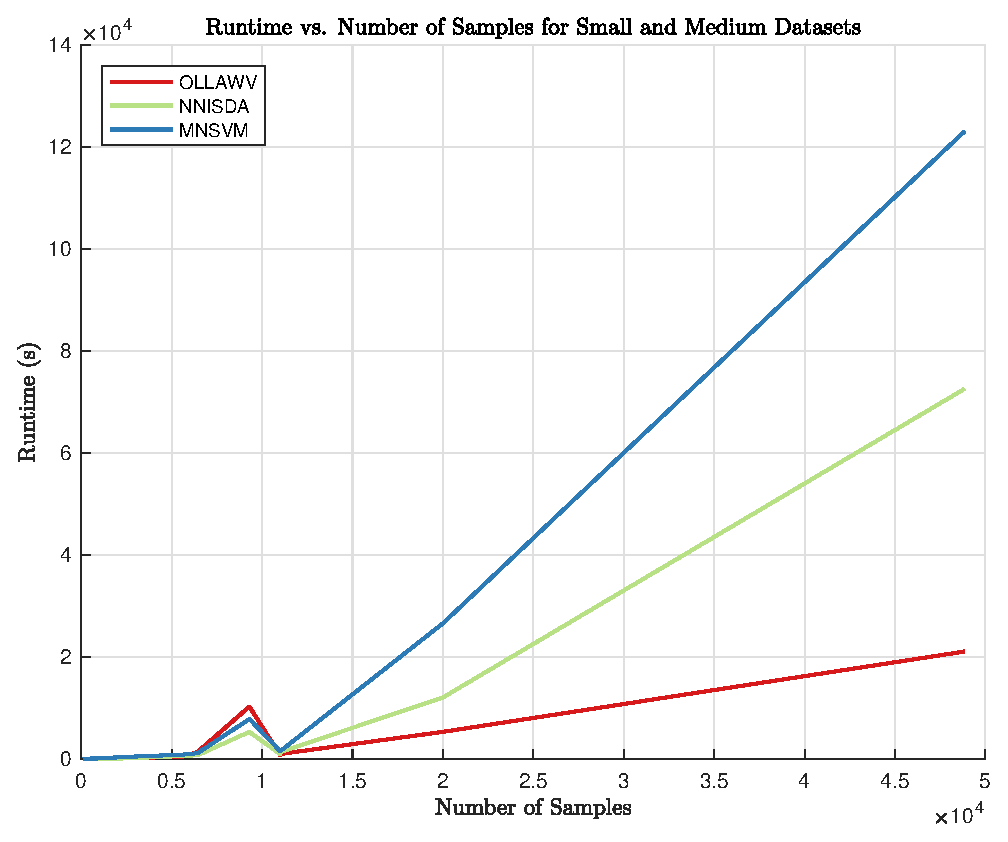
\includegraphics[width=\textwidth]{../figures/CPU_vs_NumData_SM.eps}
\end{minipage}
\begin{minipage}{0.49\textwidth}
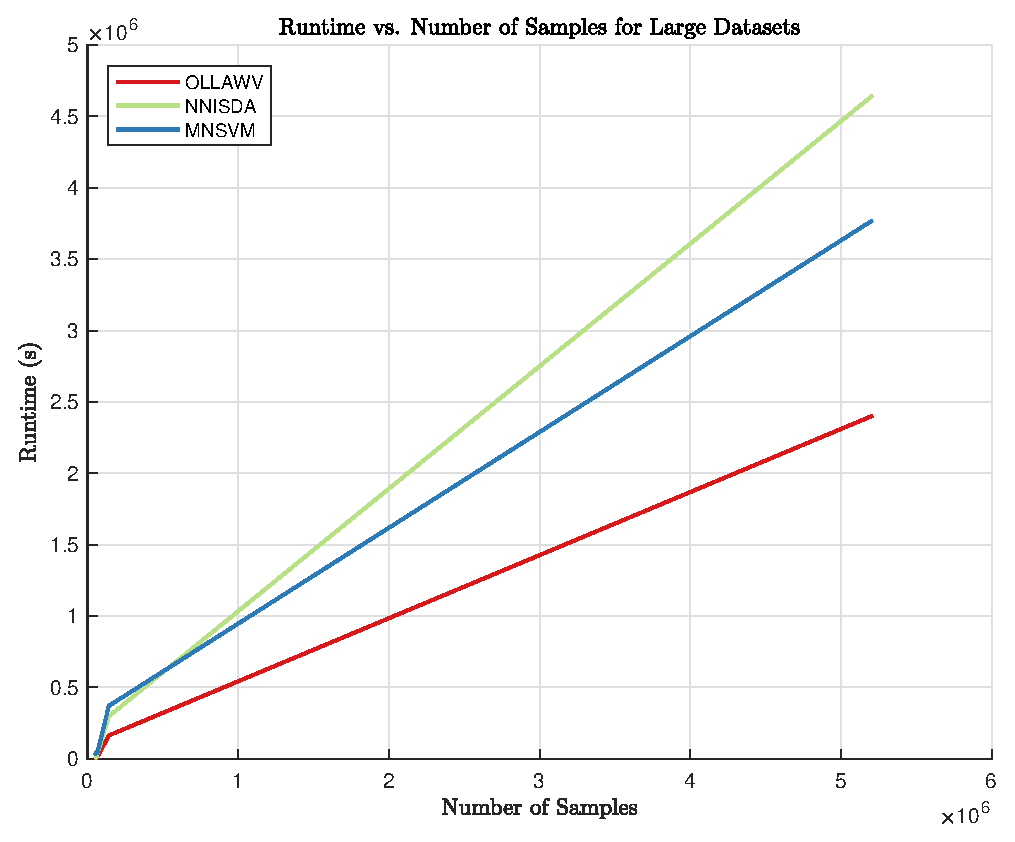
\includegraphics[width=\textwidth]{../figures/CPU_vs_NumData_L.eps}
\end{minipage}
\caption{Runtime in seconds versus the number of samples, divided into two groups: small \& medium (left) versus large (right). Note OLLAWV's gradual increase in runtime as the number of samples increases compared to NNISDA and MNSVM's steeper change. In almost all cases, OLLAWV displays superior runtime over state-of-the-art. Runtime depends upon many characteristics: dimensionality, class-overlapping, complexity of the separation boundary, number of classes as well as upon the number of support vectors, which partly explains the tiny bump in the left figure. }
\label{fig:cpuvssamples}
\end{figure}

The results in Table~\ref{tab:results} indicate that OLLAWV outperforms NNISDA and MNSVM in terms of accuracy, runtime, and model complexity. Although the differences in accuracy between the methods is not very large, on average, OLLAWV is about $2$ times faster than NNISDA and MNSVM. As mentioned previously, OLLAWV aims to speed up the learning process without sacrificing the model's accuracy. This stems from OLLAWV's ability to produce sparse models, as is shown by the averaged percentage of support vectors. The speedup that OLLAWV presents is proportional to the model complexity and the experimental results show that OLLAWV produces, on average, models that are $1.7$ times smaller than the two state-of-the-art methods used. This highlights the applicability and advantage that OLLAWV has for learning from large datasets. 

Figures~\ref{fig:BonfDunnacc}, \ref{fig:BonfDunncpu}, and \ref{fig:BonfDunnsv} show the results of the statistical analysis for accuracy, runtime, and percentage of support vectors. Figures~\ref{fig:BonfDunncpu} and~\ref{fig:BonfDunnsv} show that OLLAWV is statistically significantly better than MNSVM and NNISDA for runtime and percentage of support vectors (model size). At the same time, Figure~\ref{fig:BonfDunnacc} emphasizes what was mentioned earlier: OLLAWV is shown to speed up the learning process without sacrificing model accuracy against the state-of-the-art methods used. 

Figure~\ref{fig:cpuvssamples} plots the correlation of OLLAWV, NNISDA, and MNSVM's runtime versus number of samples for the small, medium, and large datasets. The figure clearly emphasizes the benefit of using OLLAWV for large-scale learning due to it's gradual increase in runtime as the number of samples increases in comparison to NNISDA and MNSVM. Figure~\ref{fig:psvvssamples} shows the correlation between OLLAWV, NNISDA, and MNSVM's percentage of support vectors and the number of samples for all datasets. It highlights OLLAWV's model sparseness in comparison to the competing methods, while mirroring the runtime results. 

\begin{figure}
\centering
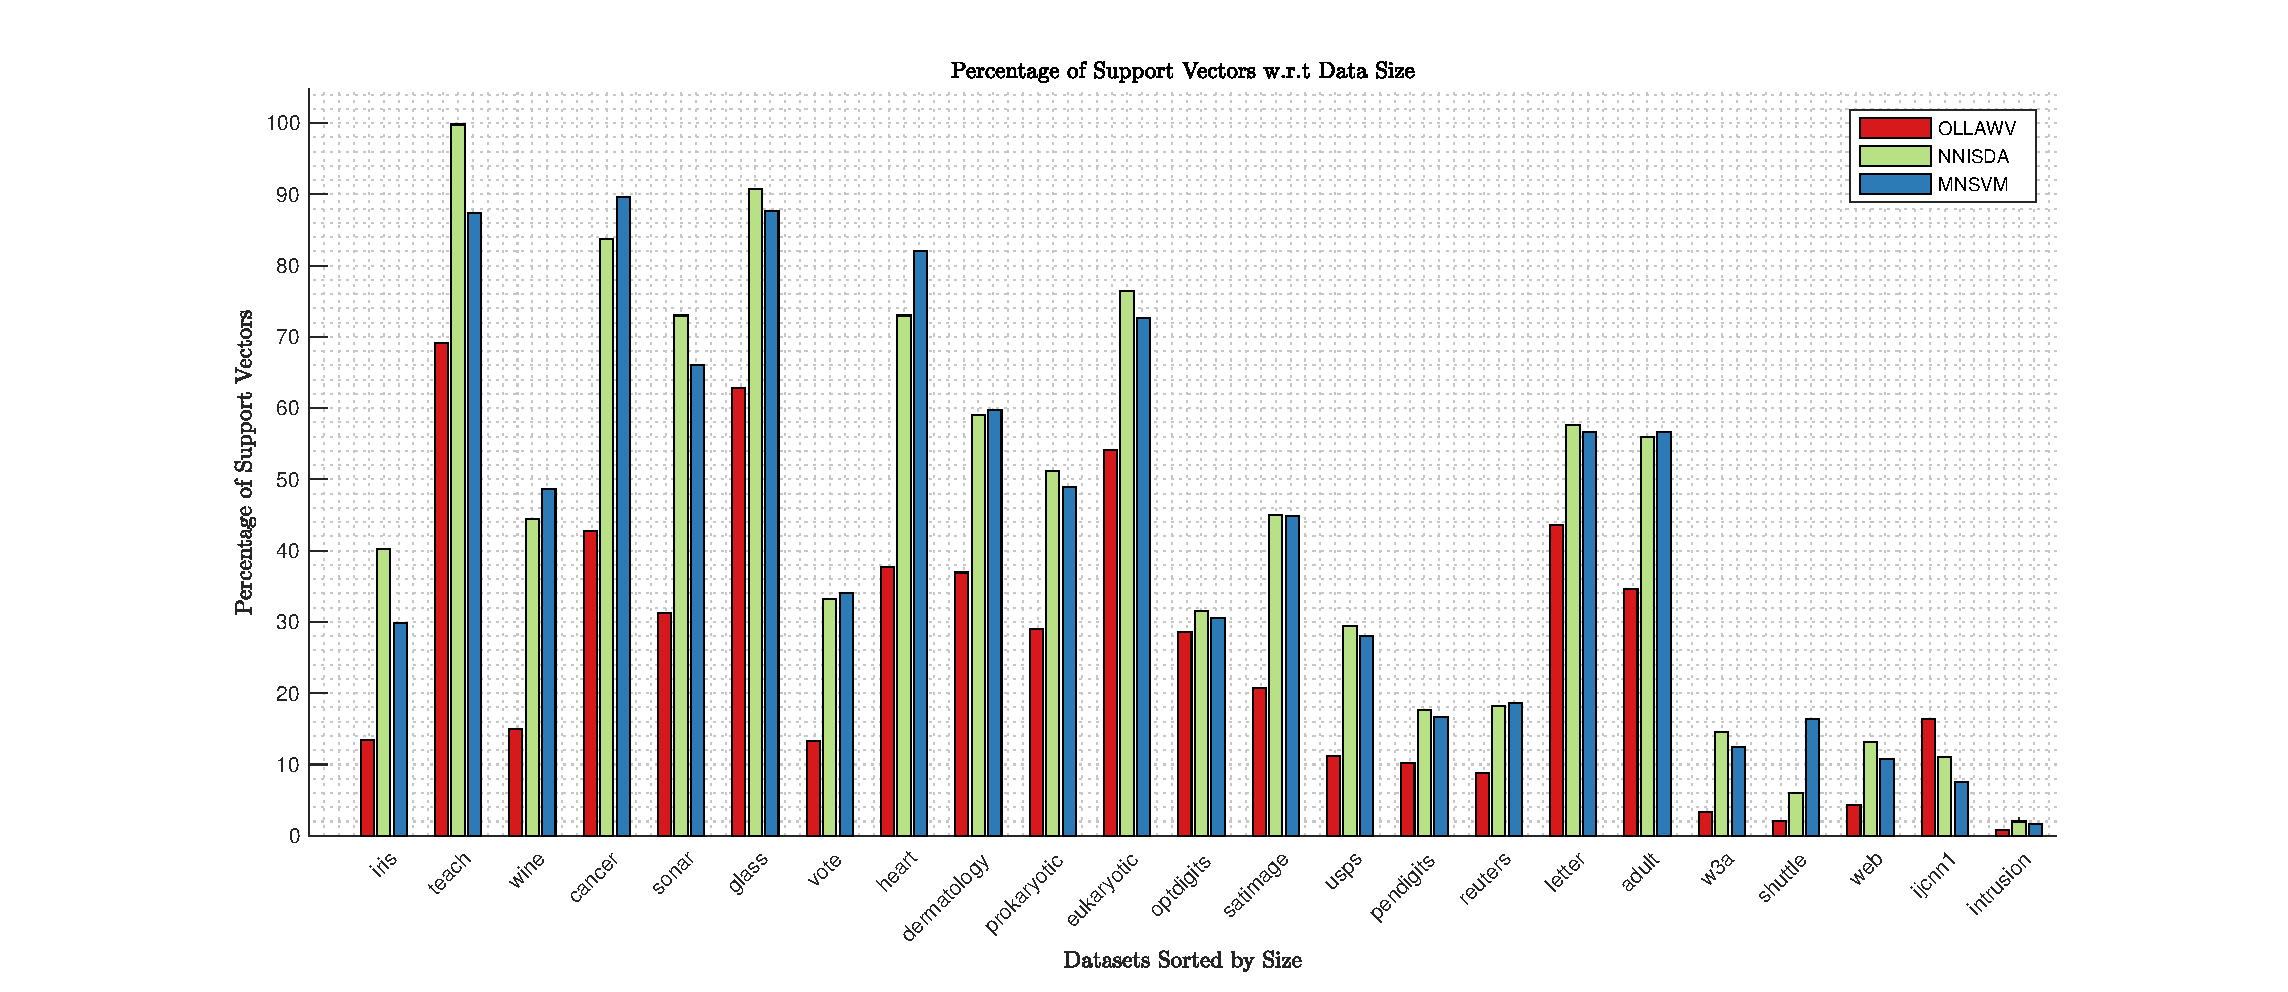
\includegraphics[trim={3.2cm 0 3.2cm 0},clip,width=\textwidth]{../figures/PSV_vs_NumData.eps}
\caption{Size of the model given as percentage of support vectors with respect to the number of samples  versus the number of samples. Note that OLLAWV’s percentage of support vectors is always smaller (except in one case) than NNISDA's and MNSVM's ones.}
\label{fig:psvvssamples}
\end{figure}

\subsection{Non-SVM Experimental Study}\label{subsec:nonsvmexp}
The supplemental experimental setup was designed to compare the performance of the proposed OLLAWV against the following $5$ popular and widely-used non-SVM algorithms: \textit{k-Nearest Neighbors (KNN)}, \textit{J48}, \textit{JRip}, \textit{Na\"ive Bayes}, and \textit{Logistic}. These methods have been implemented within the Weka framework~\cite{eibe2016weka}. The experiments were performed under the same nested $5$-fold cross-validation framework as the SVM algorithm experimental study which was described in Section~\ref{subsec:expsvm}. The following hyper-parameters shown in Table~\ref{tab:hyp} were used for the non-SVM algorithms.

\begin{table}[H]
\caption{Non-SVM Algorithm Hyper-parameters}
\label{tab:hyp}
\centering
\begin{tabular}{ll}
\noalign{\smallskip}\hline\noalign{\smallskip}
Algorithm & Parameters \\
\noalign{\smallskip}\hline\noalign{\smallskip}
$k$-NN &  Number of neighbors: $k \in \set{1,\, 3,\, 5,\, 7}$\\
J48 & Pruning: $\set{\text{True},\, \text{False}}$, Pruning Confidence: $\set{0.1,\,0.25,\,0.5}$\\
JRip & Pruning: $\set{\text{True},\, \text{False}}$  \\
Naive Bayes & Use kernel estimation: $\set{\text{True},\, \text{False}}$  \\
Logistic & Log-likelihood: $\set{1\text{e}^{-7},\, 1\text{e}^{-8},\,1\text{e}^{-9}}$  \\
\noalign{\smallskip}\hline\noalign{\smallskip}
\end{tabular}
\end{table}

\subsubsection{Results and Statistical Analysis}
%CD for alpha = 0.05 is 1.3911990032582209
\begin{table}[t!]
\caption{Accuracy Comparison for Non-SVM Methods versus OLLAWV}
\footnotesize
\centering
\label{tab:OtherResultsacc}
\begin{tabularx}{\textwidth}{l@{\extracolsep{\fill}}cccccc}
\noalign{\smallskip}\hline\noalign{\smallskip}
Dataset & OLLAWV & KNN & J48 & JRip & Na\"ive Bayes & Logistic \\
\noalign{\smallskip}\hline\noalign{\smallskip}
iris & \textbf{97.33 $\pm$ 1.49} & 96.00 $\pm$ 3.65 & 94.00 $\pm$ 2.79 & 90.67 $\pm$ 4.35 & 96.00 $\pm$ 2.79 & 97.33 $\pm$ 2.79  \\
teach & 52.32 $\pm$ 3.46 & \textbf{59.64 $\pm$ 2.89} & 49.72 $\pm$ 7.58 & 56.75 $\pm$ 9.60 & 53.75 $\pm$ 6.46 & 51.77 $\pm$ 6.68 \\
wine & \textbf{98.87 $\pm$ 1.54} & 97.73 $\pm$ 3.72 & 90.43 $\pm$ 5.83 & 93.24 $\pm$ 3.27 & 96.60 $\pm$ 3.14 & 96.05 $\pm$ 2.58 \\
cancer & \textbf{80.36 $\pm$ 5.80} & 77.32 $\pm$ 6.93 & 73.81 $\pm$ 8.57 & 73.78 $\pm$ 5.81 & 67.73 $\pm$ 5.07 & 77.32 $\pm$ 7.78 \\
sonar & \textbf{92.32 $\pm$ 3.11} & 88.99 $\pm$ 4.59 & 76.16 $\pm$ 10.6 & 75.18 $\pm$ 6.77 & 73.69 $\pm$ 7.65 & 75.18 $\pm$ 7.31 \\
glass & \textbf{72.41 $\pm$ 2.28} & 67.73 $\pm$ 5.91 & 65.06 $\pm$ 5.51 & 65.59 $\pm$ 9.66 & 49.46 $\pm$ 5.19 & 62.04 $\pm$ 5.75 \\
vote & \textbf{96.54 $\pm$ 1.87} & 92.26 $\pm$ 3.19 & 95.70 $\pm$ 2.12 & 96.54 $\pm$ 2.45 & 92.24 $\pm$ 3.24 & 93.54 $\pm$ 2.59 \\
heart2 & 82.22 $\pm$ 2.93 & 79.63 $\pm$ 5.71 & 78.52 $\pm$ 2.81 & 80.74 $\pm$ 4.06 & \textbf{84.44 $\pm$ 4.46} & 83.33 $\pm$ 3.93 \\
dermatology & \textbf{97.82 $\pm$ 0.05} & 96.18 $\pm$ 1.78 & 94.52 $\pm$ 2.21 & 91.27 $\pm$ 5.08 & 97.28 $\pm$ 1.64 & 96.98 $\pm$ 2.28 \\
pro & \textbf{88.96 $\pm$ 2.14} & 87.96 $\pm$ 3.01 & 78.54 $\pm$ 1.62 & 79.13 $\pm$ 2.78 & 62.38 $\pm$ 3.54 & 87.57 $\pm$ 2.56 \\
euk & 77.38 $\pm$ 1.96 & \textbf{81.42 $\pm$ 2.06} & 65.27 $\pm$ 2.92 & 66.42 $\pm$ 3.47 & 39.27 $\pm$ 3.43 & 69.55 $\pm$ 1.34 \\
optdigits & \textbf{99.11 $\pm$ 0.38} & 98.74 $\pm$ 0.39 & 90.87 $\pm$ 1.09 & 91.28 $\pm$ 0.40 & 92.42 $\pm$ 0.75 & 95.05 $\pm$ 0.91 \\
satimage & \textbf{91.66 $\pm$ 0.80} & 90.38 $\pm$ 0.72 & 85.64 $\pm$ 1.21 & 85.33 $\pm$ 0.77 & 85.41 $\pm$ 0.92 & 88.14 $\pm$ 1.11 \\
usps & \textbf{97.49 $\pm$ 0.22} & 97.04 $\pm$ 0.47 & 88.73 $\pm$ 0.46 & 89.20 $\pm$ 1.00 & 79.45 $\pm$ 0.59 & 91.88 $\pm$ 0.65 \\
pendigits & \textbf{99.56 $\pm$ 0.12} & 99.33 $\pm$ 0.17 & 96.24 $\pm$ 0.31 & 96.34 $\pm$ 0.41 & 88.34 $\pm$ 0.65 & 95.59 $\pm$ 0.18 \\
reuters & \textbf{98.03 $\pm$ 0.22} & 97.15 $\pm$ 0.43 & 96.90 $\pm$ 0.32 & 97.18 $\pm$ 0.44 & 93.52 $\pm$ 0.02 & 69.54 $\pm$ 0.28 \\
letter & \textbf{96.99 $\pm$ 0.21} & 95.71 $\pm$ 0.19 & 87.34 $\pm$ 0.68 & 87.02 $\pm$ 0.66 & 74.12 $\pm$ 0.97 & 77.45 $\pm$ 0.16 \\
adult & \textbf{84.75 $\pm$ 0.26} & 83.85 $\pm$ 0.28 & 84.38 $\pm$ 0.28 & 83.73 $\pm$ 0.17 & 80.57 $\pm$ 0.09 & 82.46 $\pm$ 0.14 \\
w3a & \textbf{98.86 $\pm$ 0.04} & 98.60 $\pm$ 0.06 & 98.71 $\pm$ 0.05 & 98.41 $\pm$ 0.10 & 96.71 $\pm$ 0.20 & 98.61 $\pm$ 0.12 \\
shuttle & 99.77 $\pm$ 0.03 & 99.93 $\pm$ 0.03 & \textbf{99.97 $\pm$ 0.02} & 99.96 $\pm$ 0.02 & 98.57 $\pm$ 0.24 & 96.83 $\pm$ 0.12 \\
web & \textbf{98.94 $\pm$ 0.05} & 98.89 $\pm$ 0.06 & 98.79 $\pm$ 0.09 & 98.50 $\pm$ 0.13 & 96.71 $\pm$ 0.21 & 98.70 $\pm$ 0.08 \\
ijcnn1 & 98.31 $\pm$ 0.07 & \textbf{98.48 $\pm$ 0.04} & 98.40 $\pm$ 0.09 & 98.11 $\pm$ 0.10 & 90.69 $\pm$ 0.26 & 92.29 $\pm$ 0.16 \\
intrusion & \textbf{99.77 $\pm$ 0.02} & 88.20 $\pm$ 1.06 & 58.01 $\pm$ 26.6 & 87.66 $\pm$ 3.79 & 49.75 $\pm$ 30.7 & 65.15 $\pm$ 15.7 \\
\noalign{\smallskip}\hline\noalign{\smallskip}
Average & \textbf{91.29 $\pm$ 1.26} & 90.05 $\pm$ 2.06 & 84.60 $\pm$ 3.64 & 86.18 $\pm$ 2.84 & 79.96 $\pm$ 3.58 & 84.45 $\pm$ 2.83 \\
Ranks & \textbf{1.500} & $2.500$ & $4.041$ & $3.9583$ & $5.0625$ & $3.9375$ \\
\noalign{\smallskip}\hline\noalign{\smallskip}
\end{tabularx}
\begin{minipage}{0.9\textwidth}
\centering
\vspace{1em}
\resizebox{0.9\textwidth}{!}{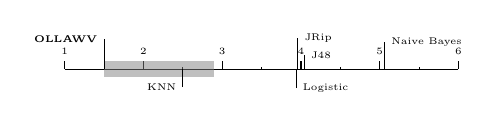
\begin{tikzpicture}
\draw (1,0) -- (6,0);
\foreach \x in {1,2,3,4,5,6} {
\draw (\x, 0) -- ++(0,.1) node [above,scale=0.7] {\tiny \x};
\ifthenelse{\x < 6}{\draw (\x+.5, 0) -- ++(0,.03);}{}
}

\coordinate (c0) at (1.5,0);
\coordinate (c1) at (2.5,0);
\coordinate (c2) at (4.041,0);
\coordinate (c3) at (3.9583,0);
\coordinate (c4) at (5.0625,0);
\coordinate (c5) at (3.9375,0);

\node (l0) at (c0) [above left=.25cm and 0cm, align=right,scale=0.7] {\tiny \textbf{OLLAWV}};
\node (l1) at (c1) [below left=.1cm and 0cm, align=right,scale=0.7] {\tiny KNN};
\node (l2) at (c2) [above right=.05cm and 0cm, align=right,scale=0.7] {\tiny J48};
\node (l3) at (c3) [above right=.25cm and 0cm, align=right,scale=0.7] {\tiny JRip};
\node (l4) at (c4) [above right=.2cm and 0cm, align=right,scale=0.7] {\tiny Naive Bayes};
\node (l5) at (c5) [below right=.1cm and 0cm, align=right,scale=0.7] {\tiny Logistic};


\fill[fill=gray,fill opacity=0.5] (1.5,-0.1) rectangle (2.89,0.1);

\foreach \x in {0,1,2,3,4,5} {
\draw (l\x) -| (c\x);
};
\end{tikzpicture}}
\captionsetup{width=0.8\linewidth}
\captionof{figure}{Bonferroni-Dunn test for Accuracy}\label{fig:BonfDunnaccOther}
\end{minipage}
\vspace{-1em}
\end{table}

\begin{figure}
\centering
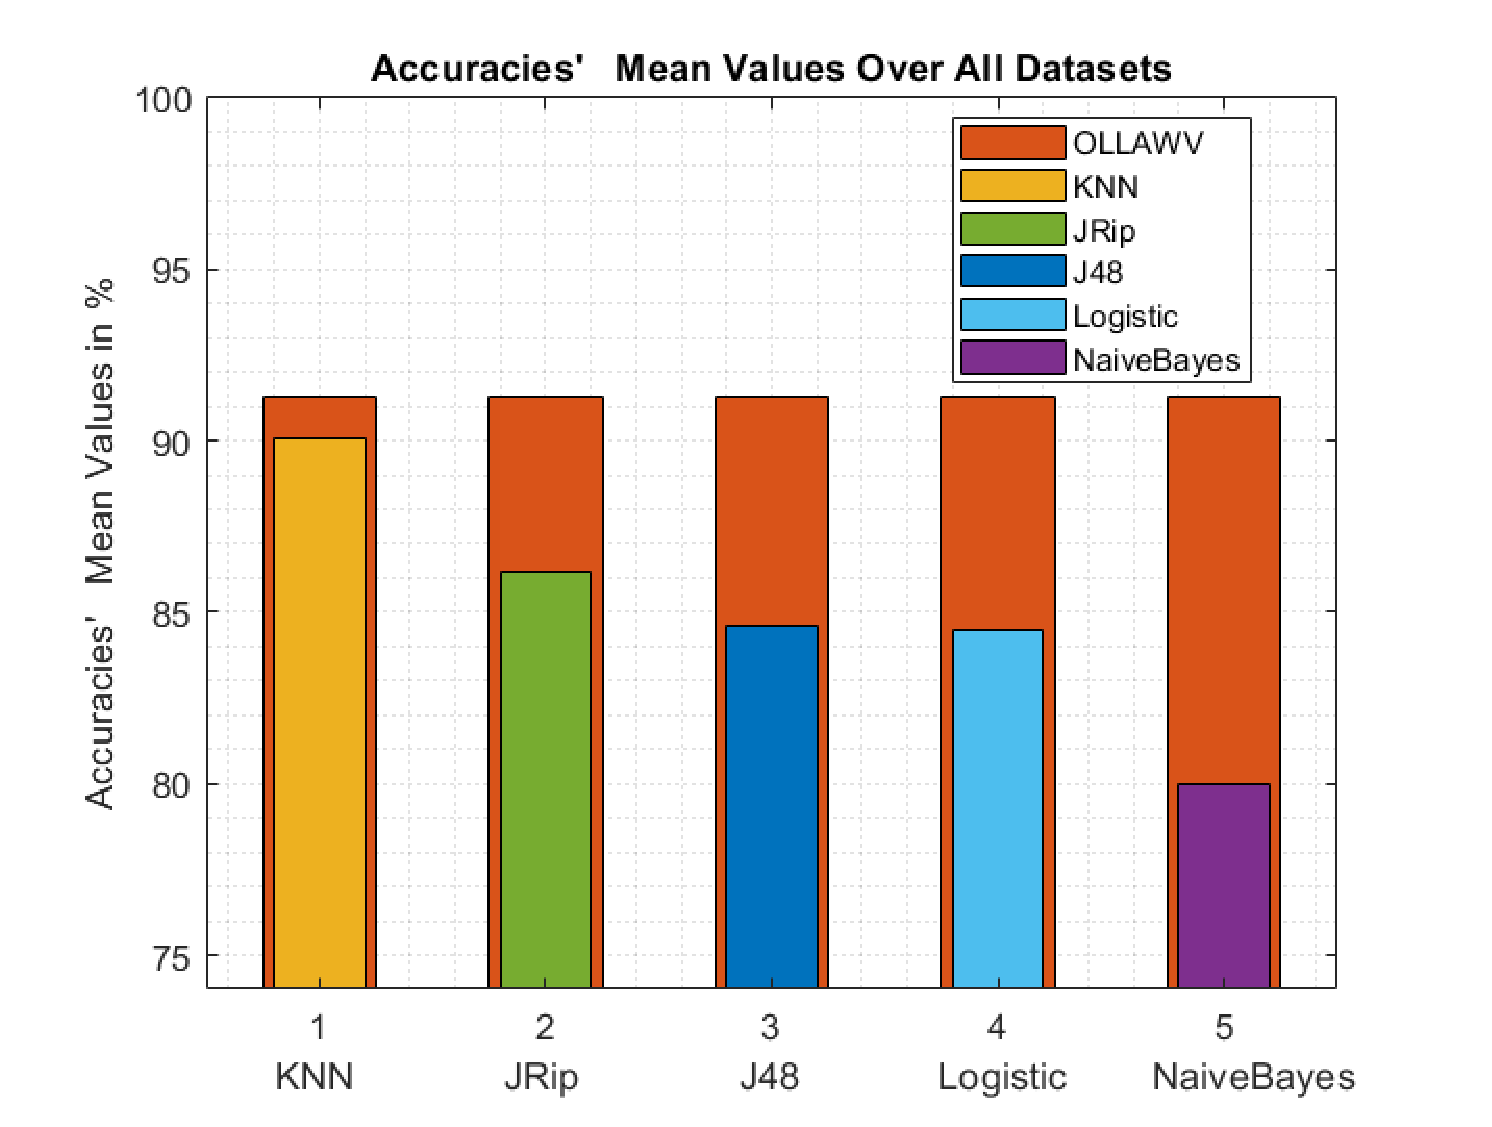
\includegraphics[width=0.6\textwidth]{../figures/others.eps}
\caption{Mean accuracy over all datasets for OLLAWV and the 5 non-SVM state-of-the-art methods.}
\label{fig:accother}
\end{figure}
Table~\ref{tab:OtherResultsacc} displays the accuracy results for OLLAWV and five state-of-the-art methods. The table also shows the standard deviation for accuracy per outer fold, the average values accross all datasets, and the algorithm ranks. As the results indicate, OLLAWV outperforms all other state-of-the-art methods. Figure~\ref{fig:accother} displays the average accuracy results for OLLAWV and the non-SVM methods accross all datasets and highlights OLLAWV's better performance. The Friedman test indicates that OLLAWV performs significantly better than the competing methods for $\alpha = 0.05$ and is ranked first. Figure~\ref{fig:BonfDunnaccOther} shows the critical distance bar (which is $1.391$), and indicates that all other algorithms perform statistically significantly worse than OLLAWV, except for KNN. 

\section{Conclusion}\label{sec:conclusion}
This paper proposed a novel online learning procedure and algorithm for solving the L1-SVM problem, which is a unique method in terms of both iterating over samples and updating the model. A new stopping criterion for the stochastic gradient procedure is also proposed. The model is updated by changing the weight $\alpha_i$ of a single worst-violator per iteration and stops when all violating samples i.e., support vectors, are found. Finding the \textit{worst-violators} is done without replacement. Such an approach results in a significant shortening of training time, as well as in a huge decrease in the resulting model size. The key features of the proposed algorithm, OLLAWV, stem from it's implicit ability of finding support vectors and it's self-stopping condition. This design was devised to address the limitations presented by current SVM solvers. 

The first experimental study demonstrates the better performance of OLLAWV compared with state-of-the-art SVM solvers (MNSVM and NNISDA) which have been shown to outperform the popular SMO implementation in the LIBSVM package. The results for accuracy, runtime, and percentage of support-vectors, obtained by the strict nested cross-validation procedure, were compared and further validated using statistical analysis with non-parametric tests. They highlighted the advantages and major speedup achieved by OLLAWV against the competing MNSVM and NNISDA. The second, supplemental experimental study evaluated the performance of OLLAWV against $5$ popular non-SVM methods, showing the better performance of OLLAWV against all five non-SVM algorithms ($k$-Nearest Neighbors (KNN), J48, JRip, Na\"ive Bayes, and Logistic). The proposal, OLLAWV, performs statistically better in terms of runtime and model size across all $23$ evaluated benchmark datasets, without compromising accuracy.


\end{document}